
In this section we will look at the results of the models proposed in Section \ref{sec:methods}. 


\subsection{Training Metrics}
First we show loss curves during training on train and validation data of the different diffusion model types, see Figure \ref{fig:losscurvesall}.



We observe that no models have any problems with over-fitting. The CNN based models overall performs best with regards towards minimizing the train loss.

% \begin{figure}[t]
%     \centering
%     \subfloat[train]{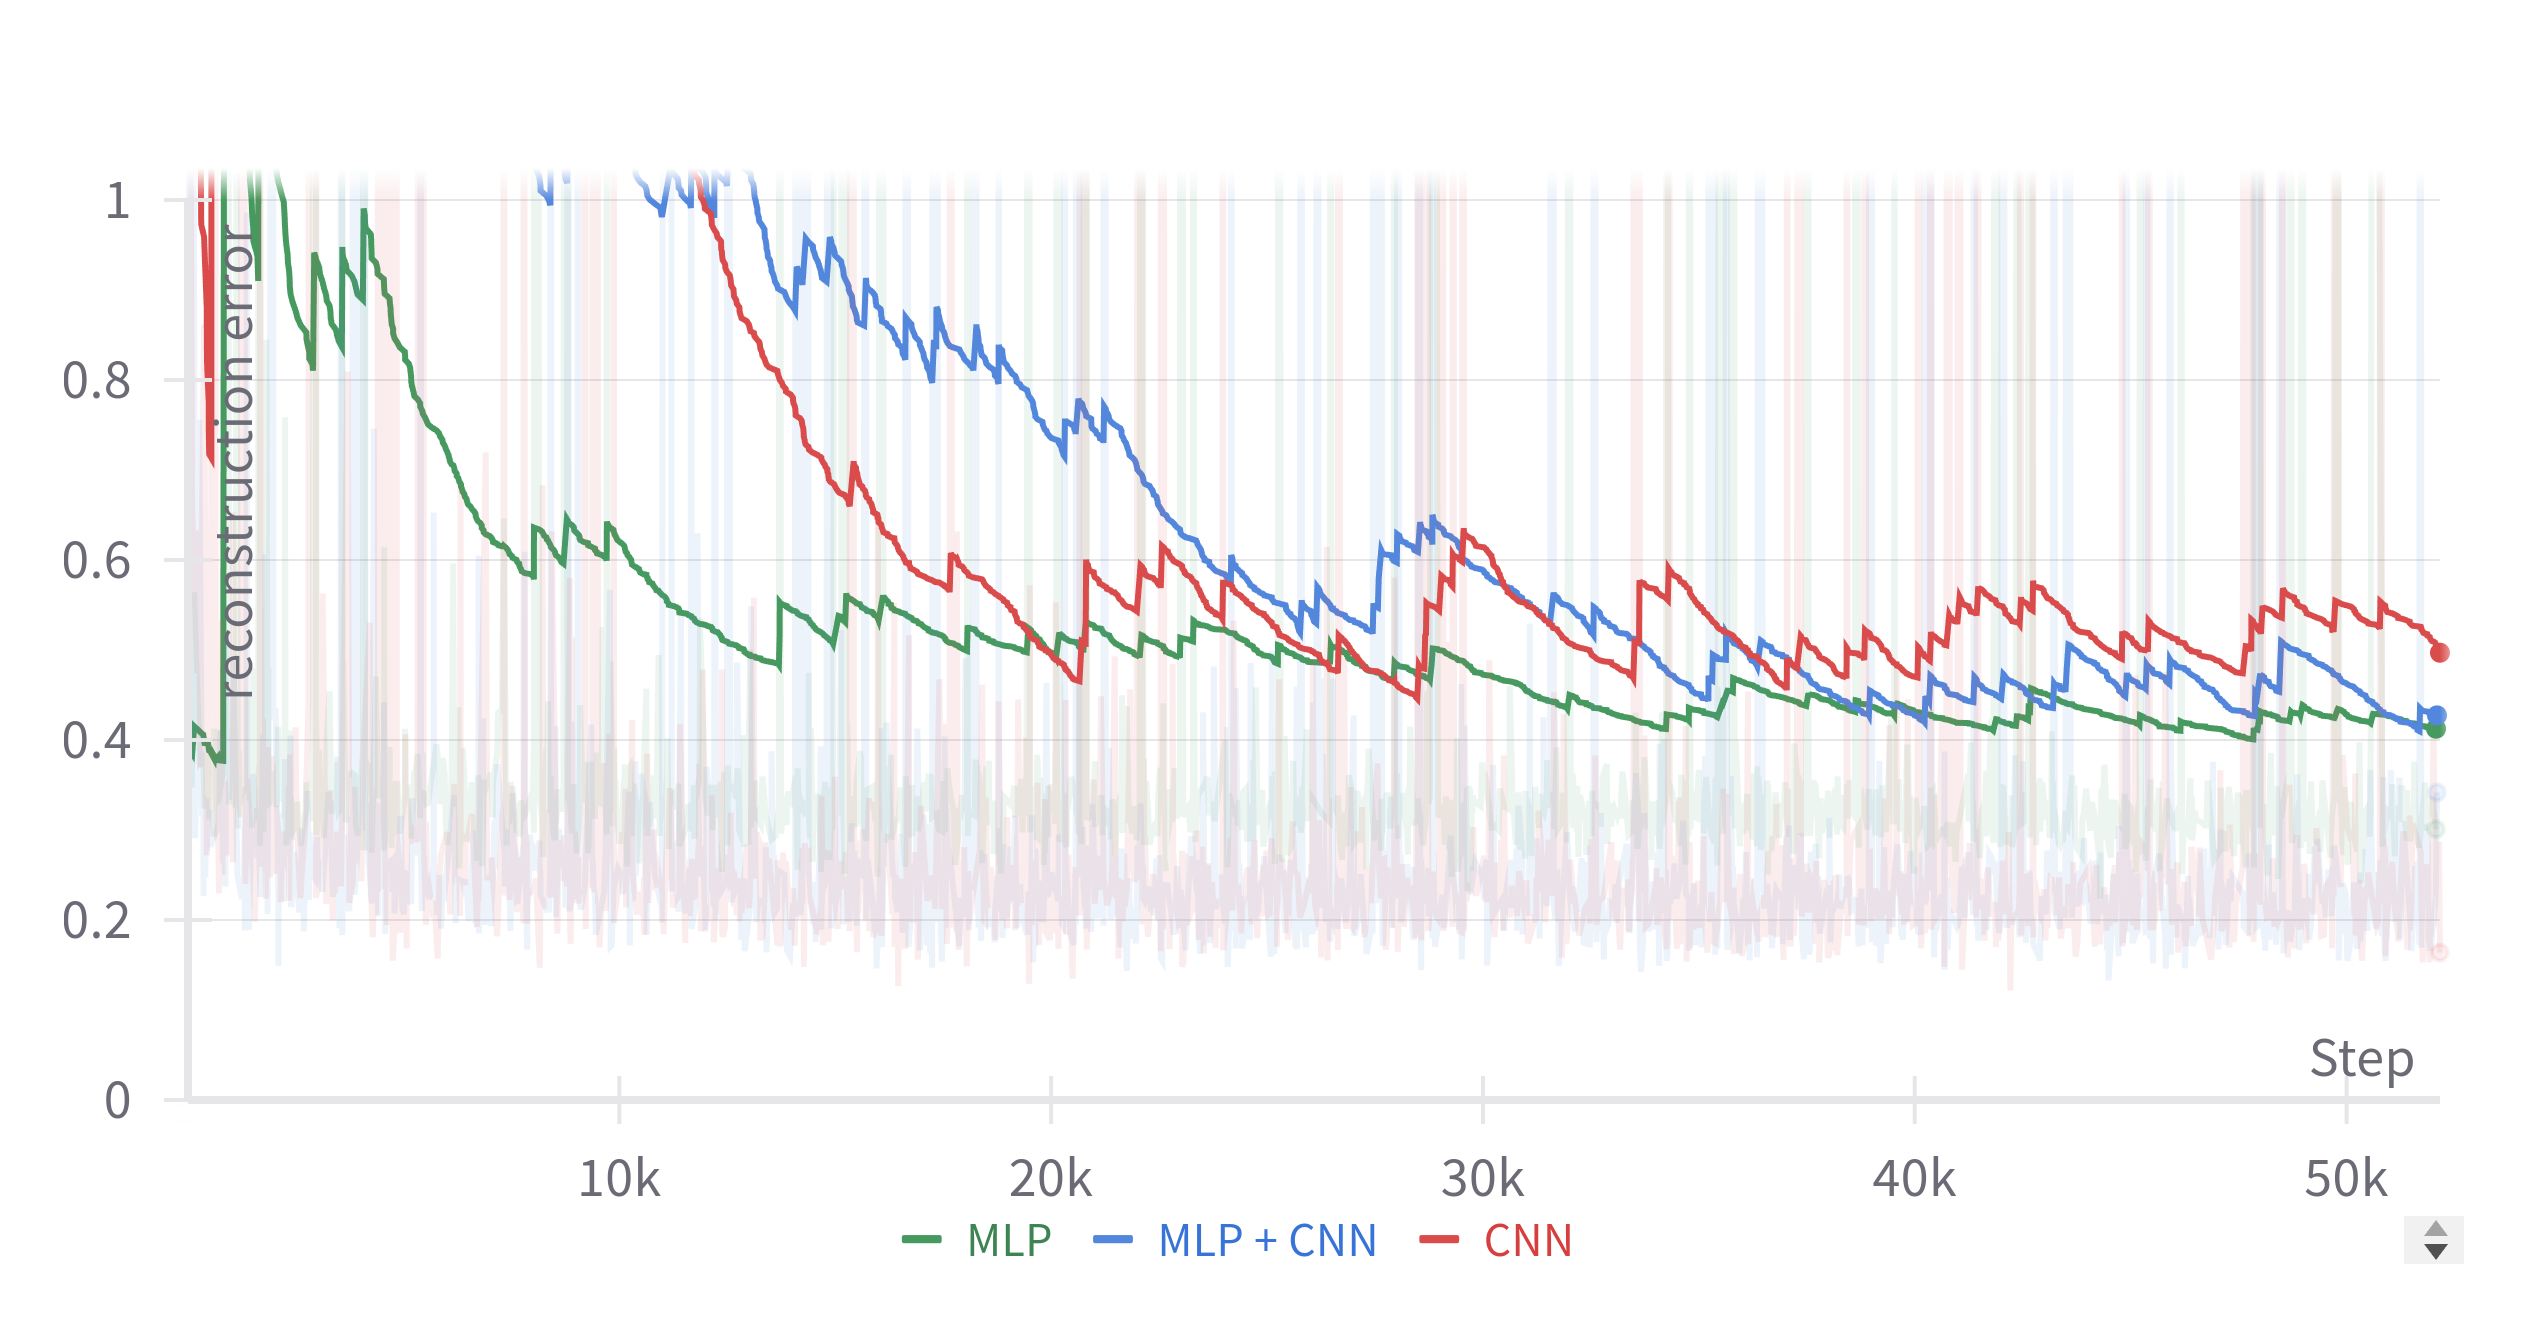
\includegraphics[width = 0.33\textwidth]{figures/reconstruction_error.png}}
%     \subfloat[validation]{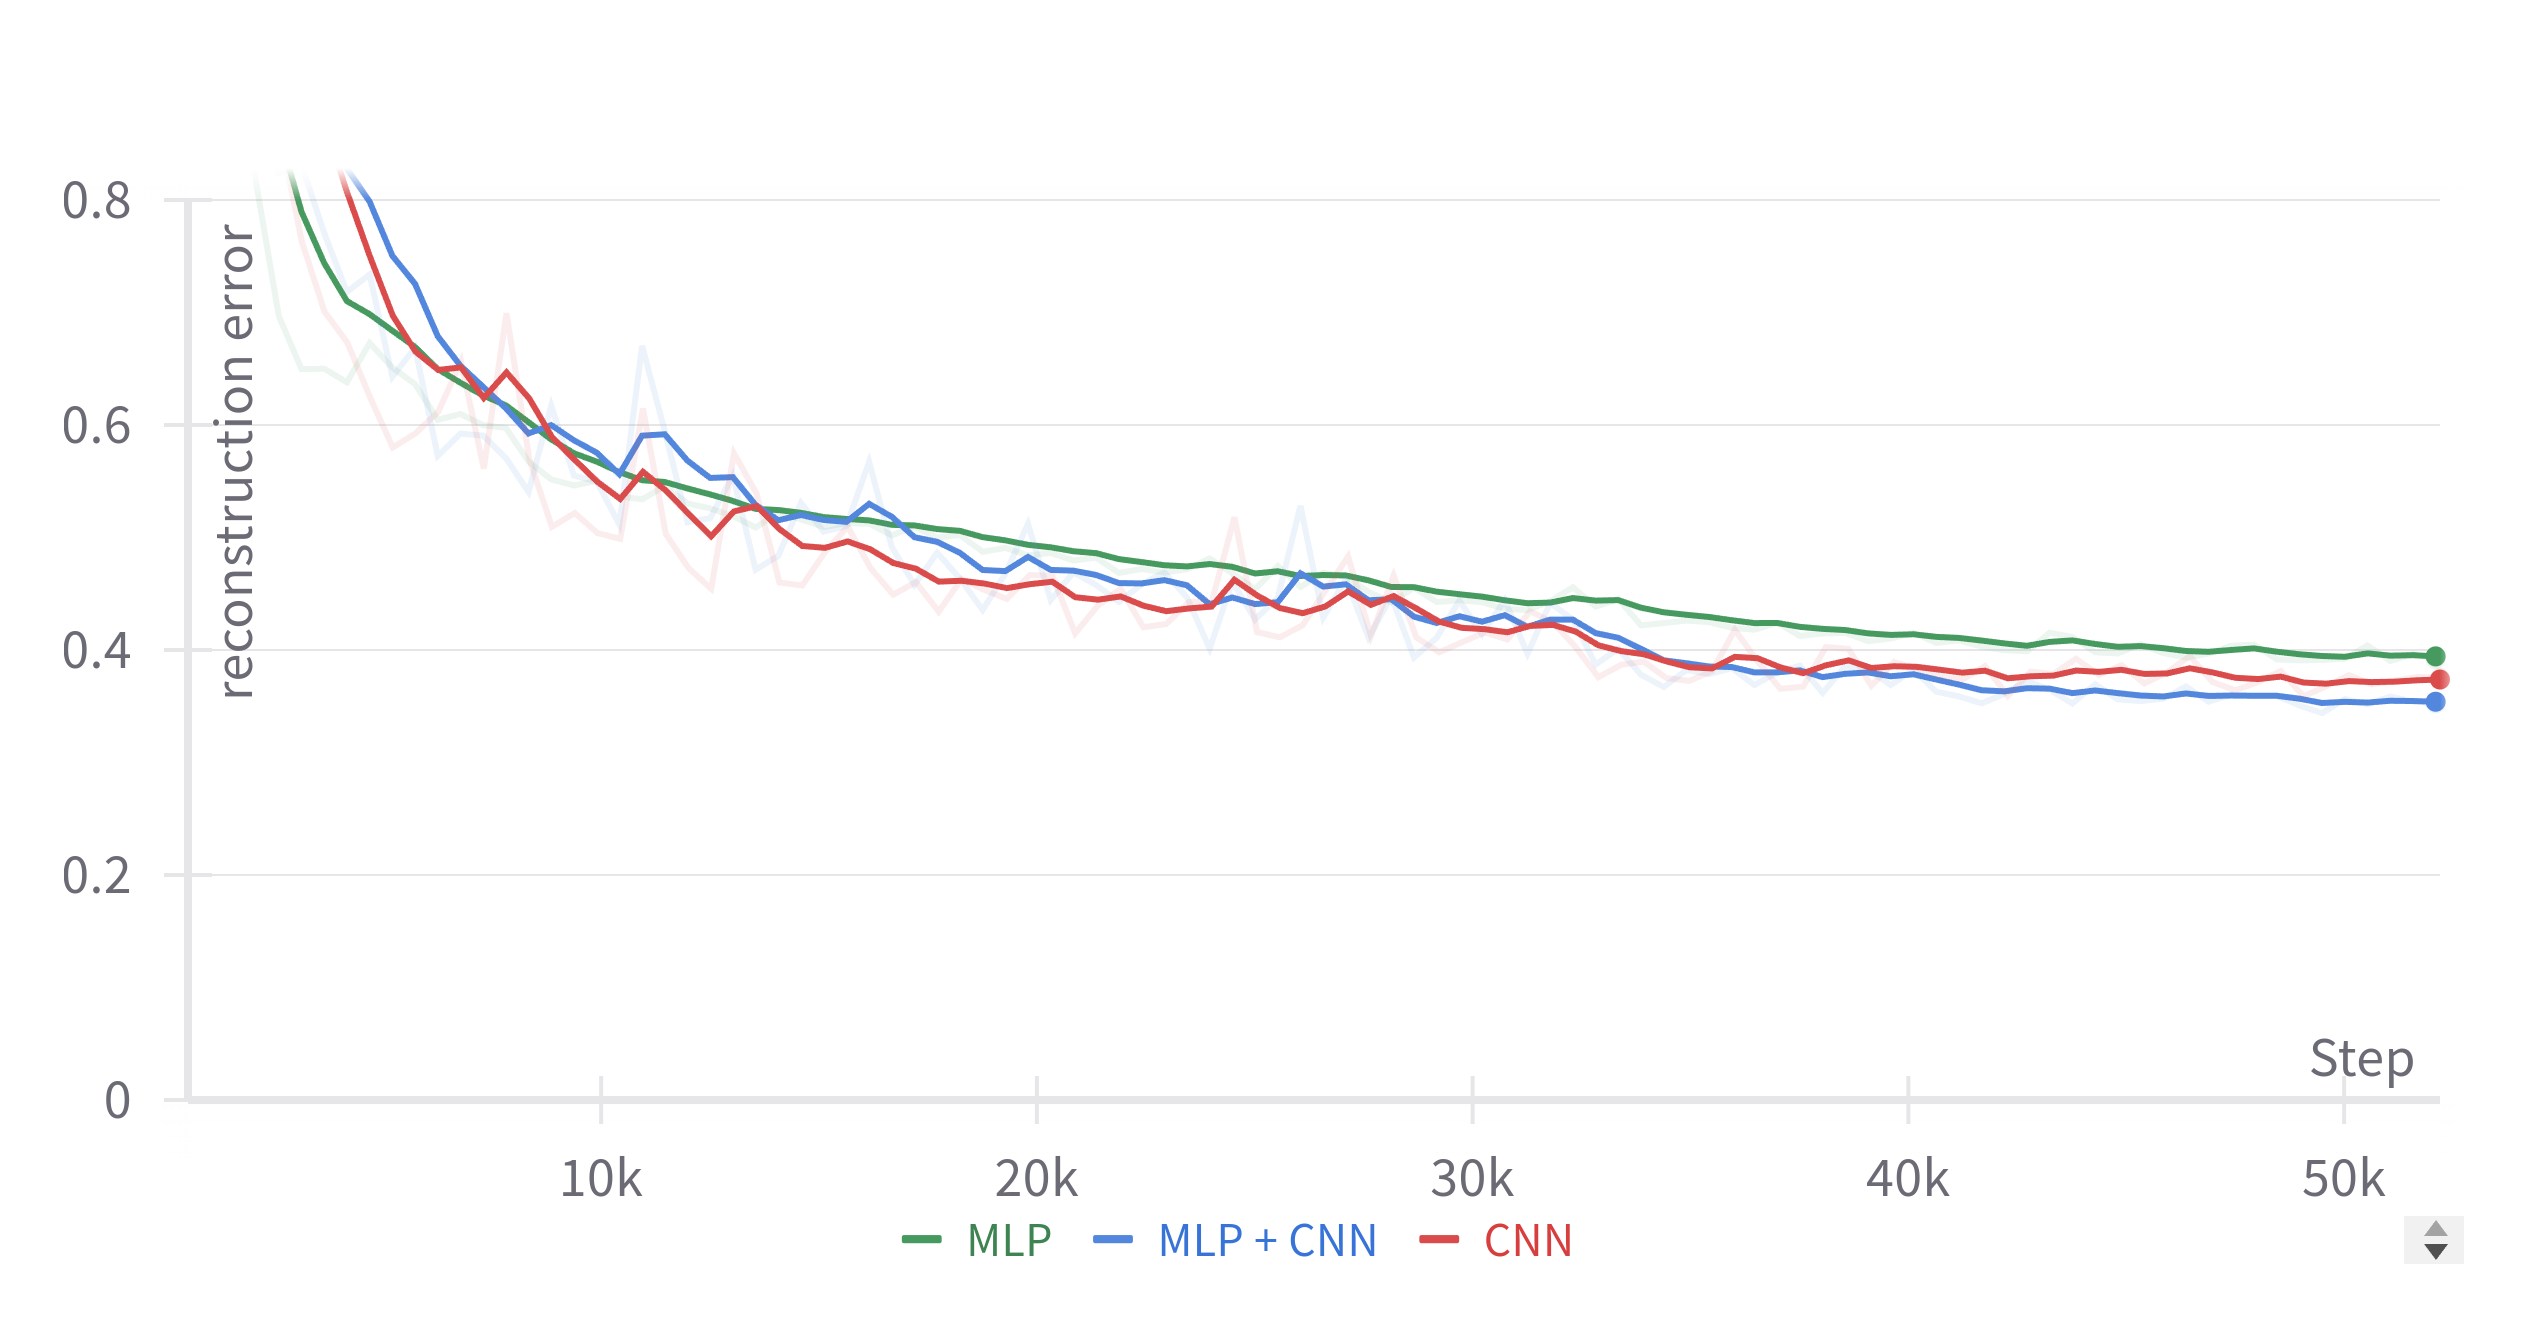
\includegraphics[width = 0.33\textwidth]{figures/valrecerror (1).png}}  

%     \caption{}
%     \label{fig:recerror}
% \end{figure}



However, if we take a closer look at the reconstruction error of the model, visualized in Figure \ref{fig:losscurvesall}, we note that the MLP model actually performs surprisingly similar to the CNN model and that even though only very small drops in loss during training can be observed for the MLP, the reconstruction error keeps improving. The Transformer based architecture seems to be performing decently in loss and reconstruction error.
We note that reconstruction error is highly related to the loss, but scaled by the noise schedule $t$, e.g. this error focuses more on large values of $t$.

To further analyze this, in Figure \ref{fig:lossvsnoise} we visualize the reconstruction error curves vs amount of noise added of the different diffusion models. We can see that while the CNN has an overall better performance it focuses more on the fine detail of the structure e.g. recovering from small noise values, while the MLP architecture is more focused on recovering rough structure (e.g. high noise). 
\begin{wrapfigure}{r}{0.5\textwidth}
  \centering
  \subfloat[train loss]{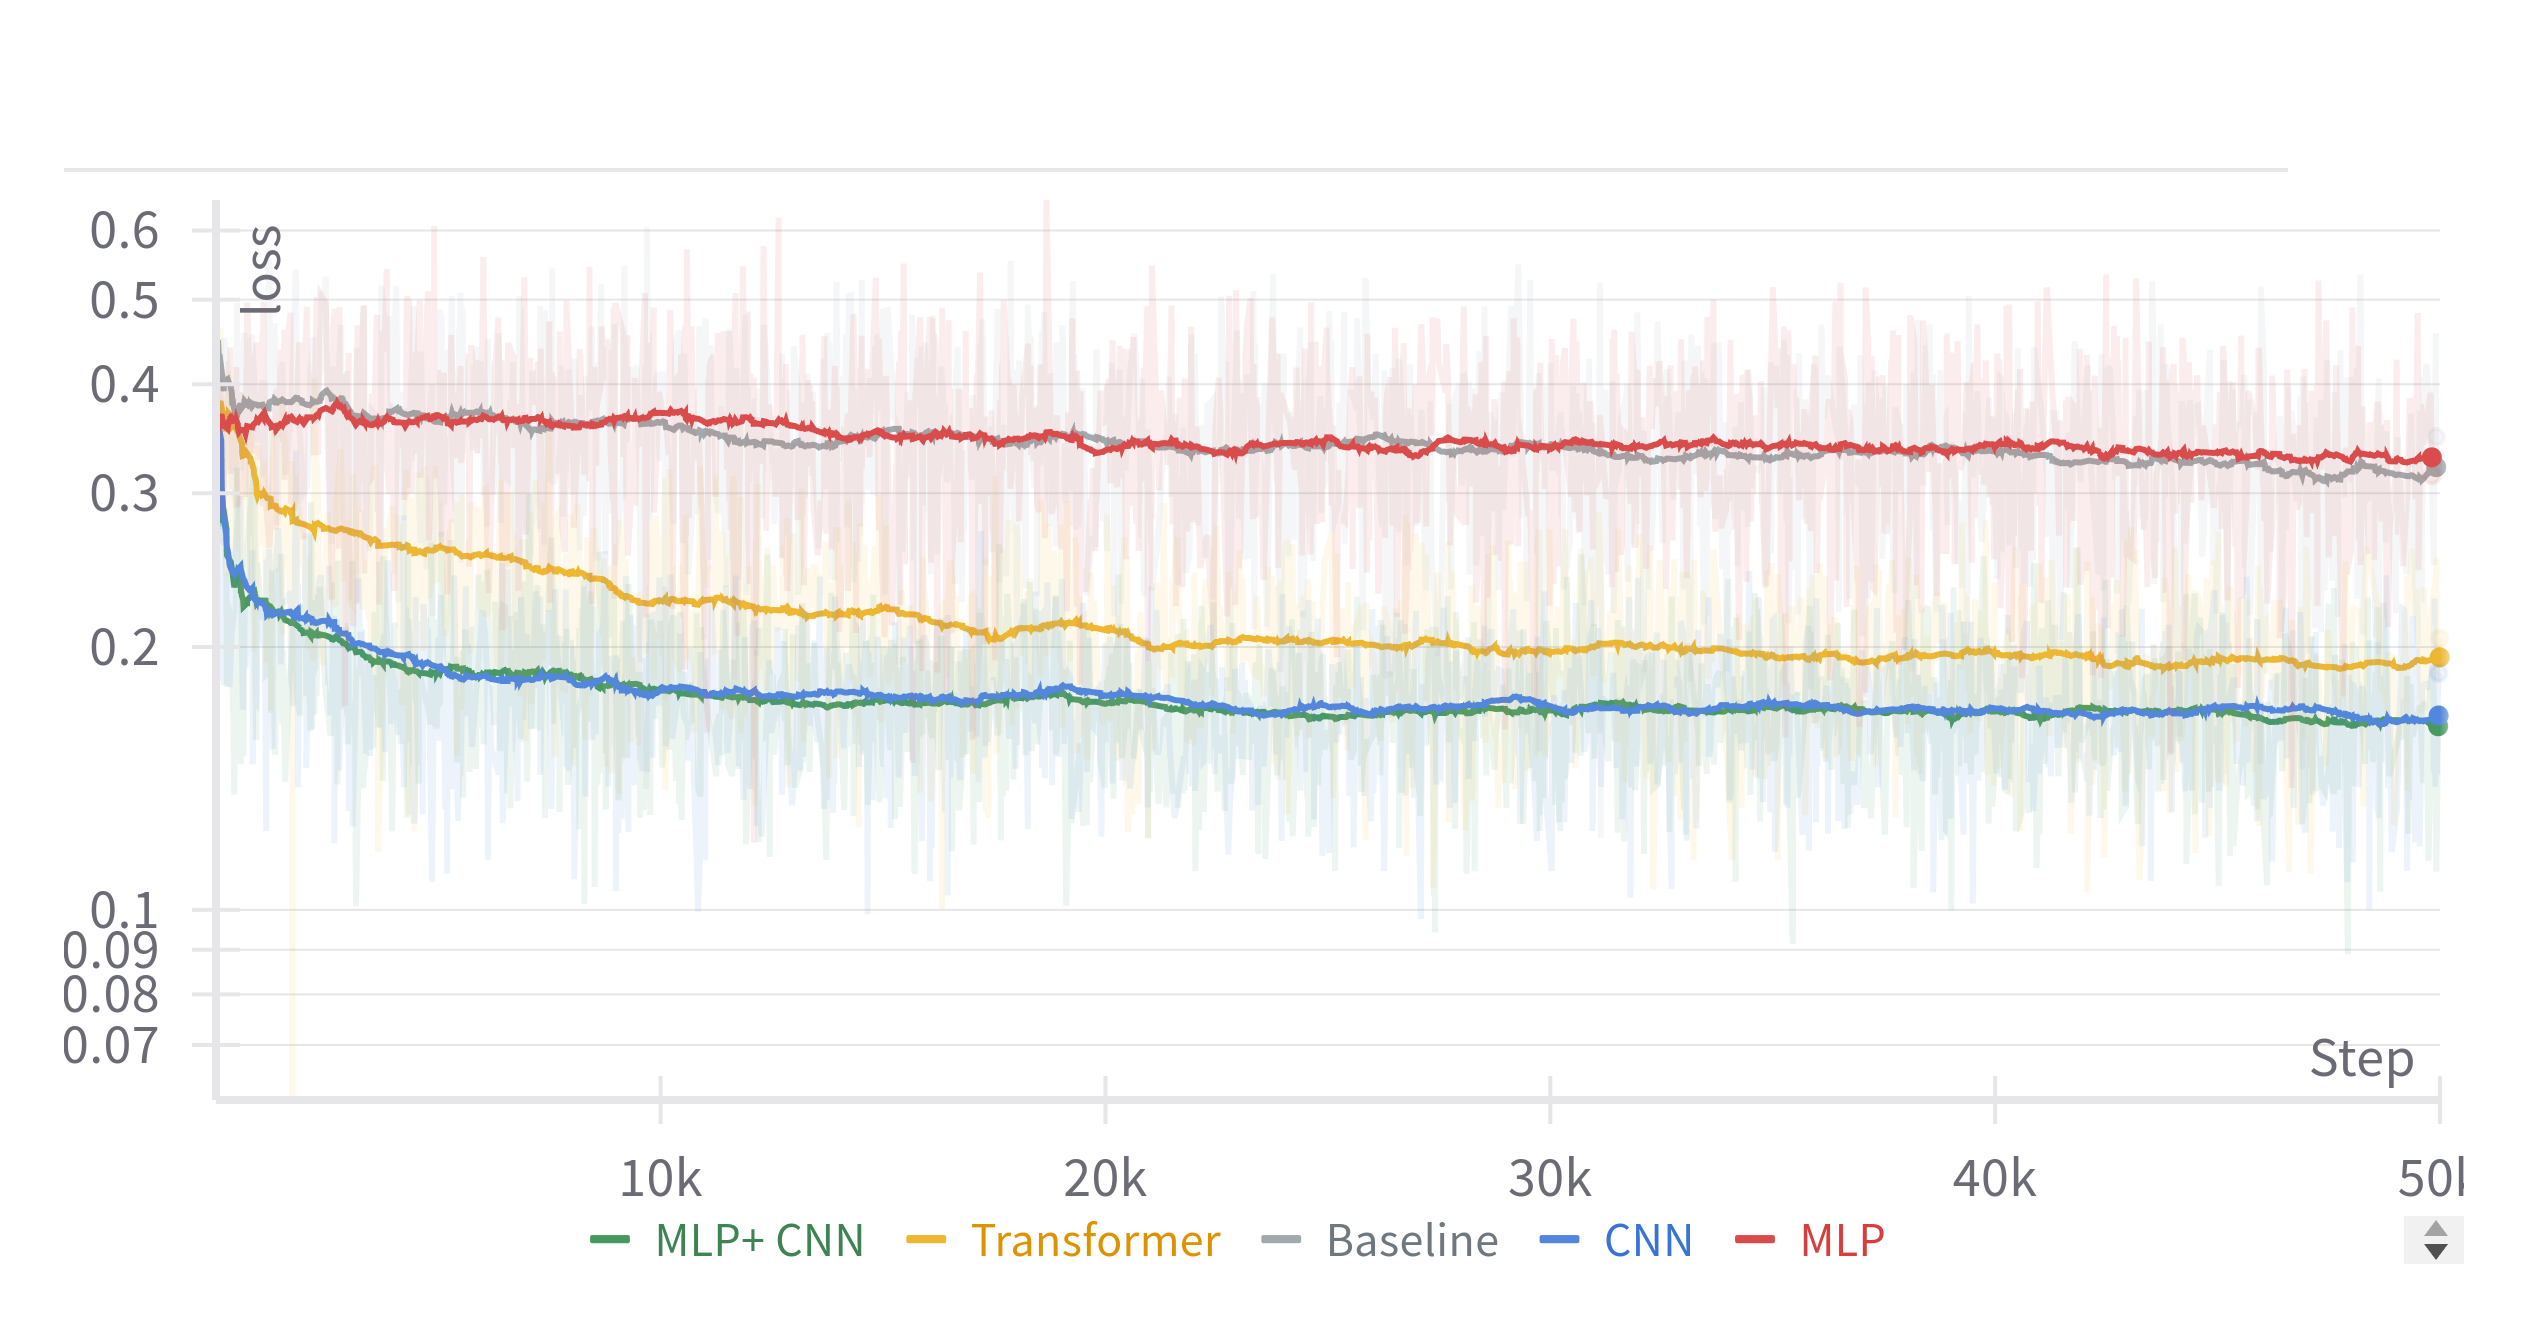
\includegraphics[width = 0.25\textwidth]{figures/losstrain.png}}
  \subfloat[validation loss]{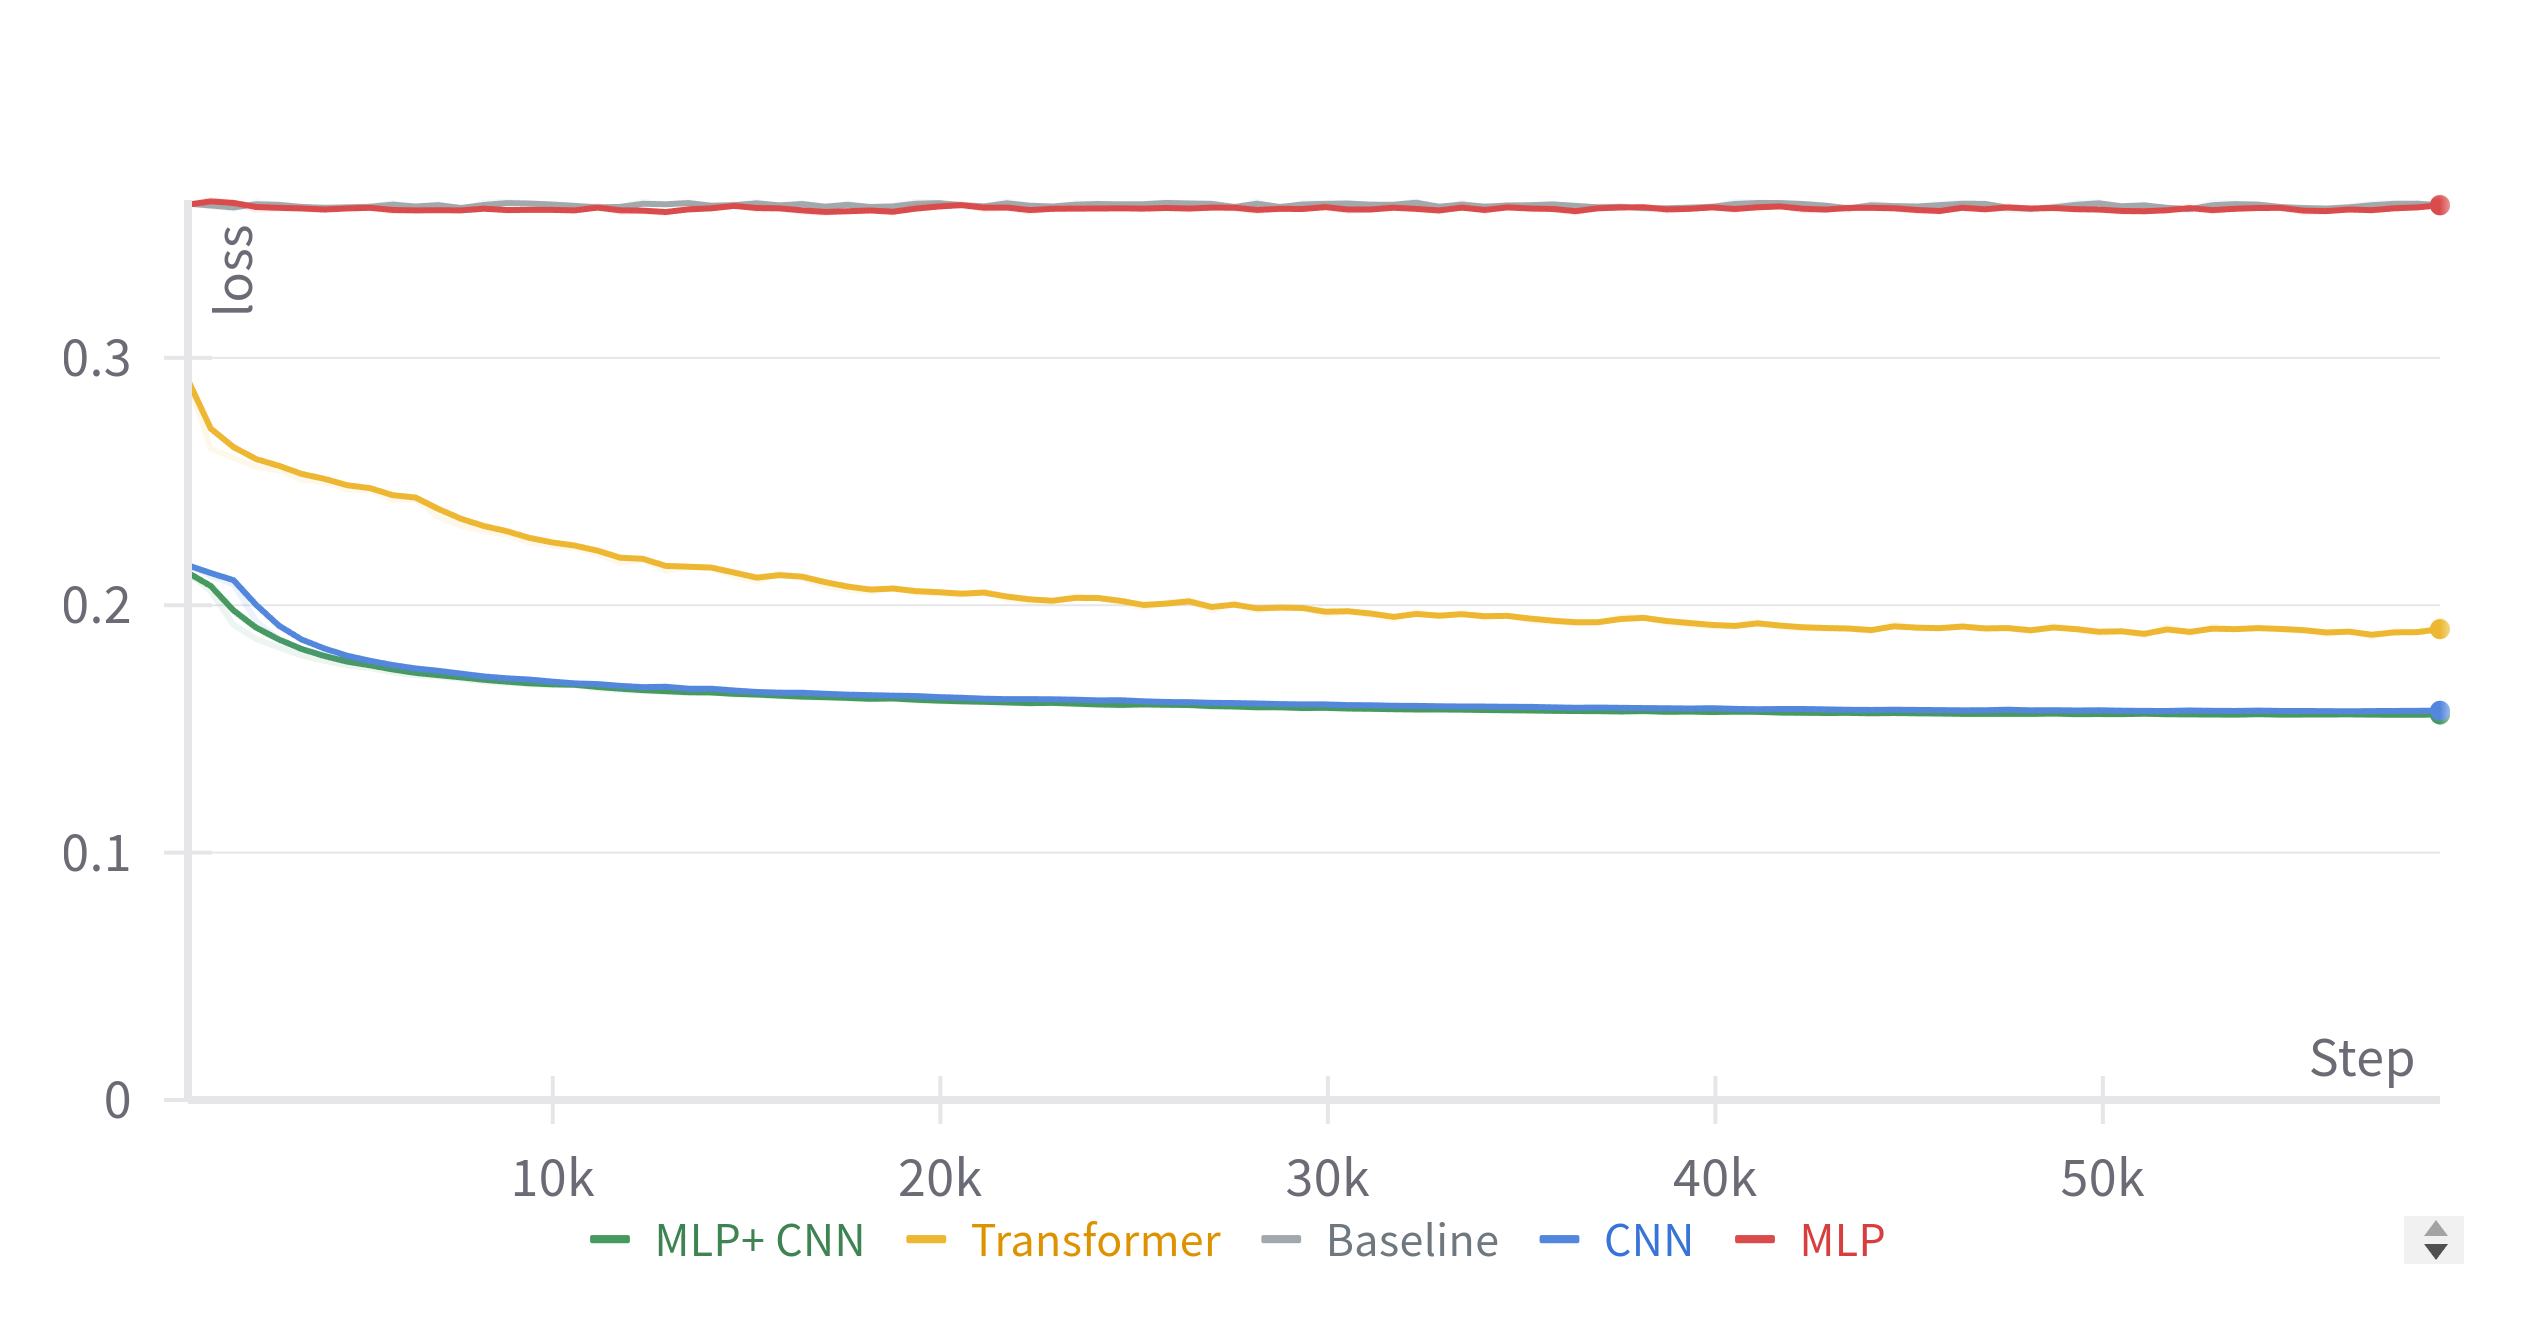
\includegraphics[width = 0.25\textwidth]{figures/lossval.png}}   \\

  \subfloat[train rec error]{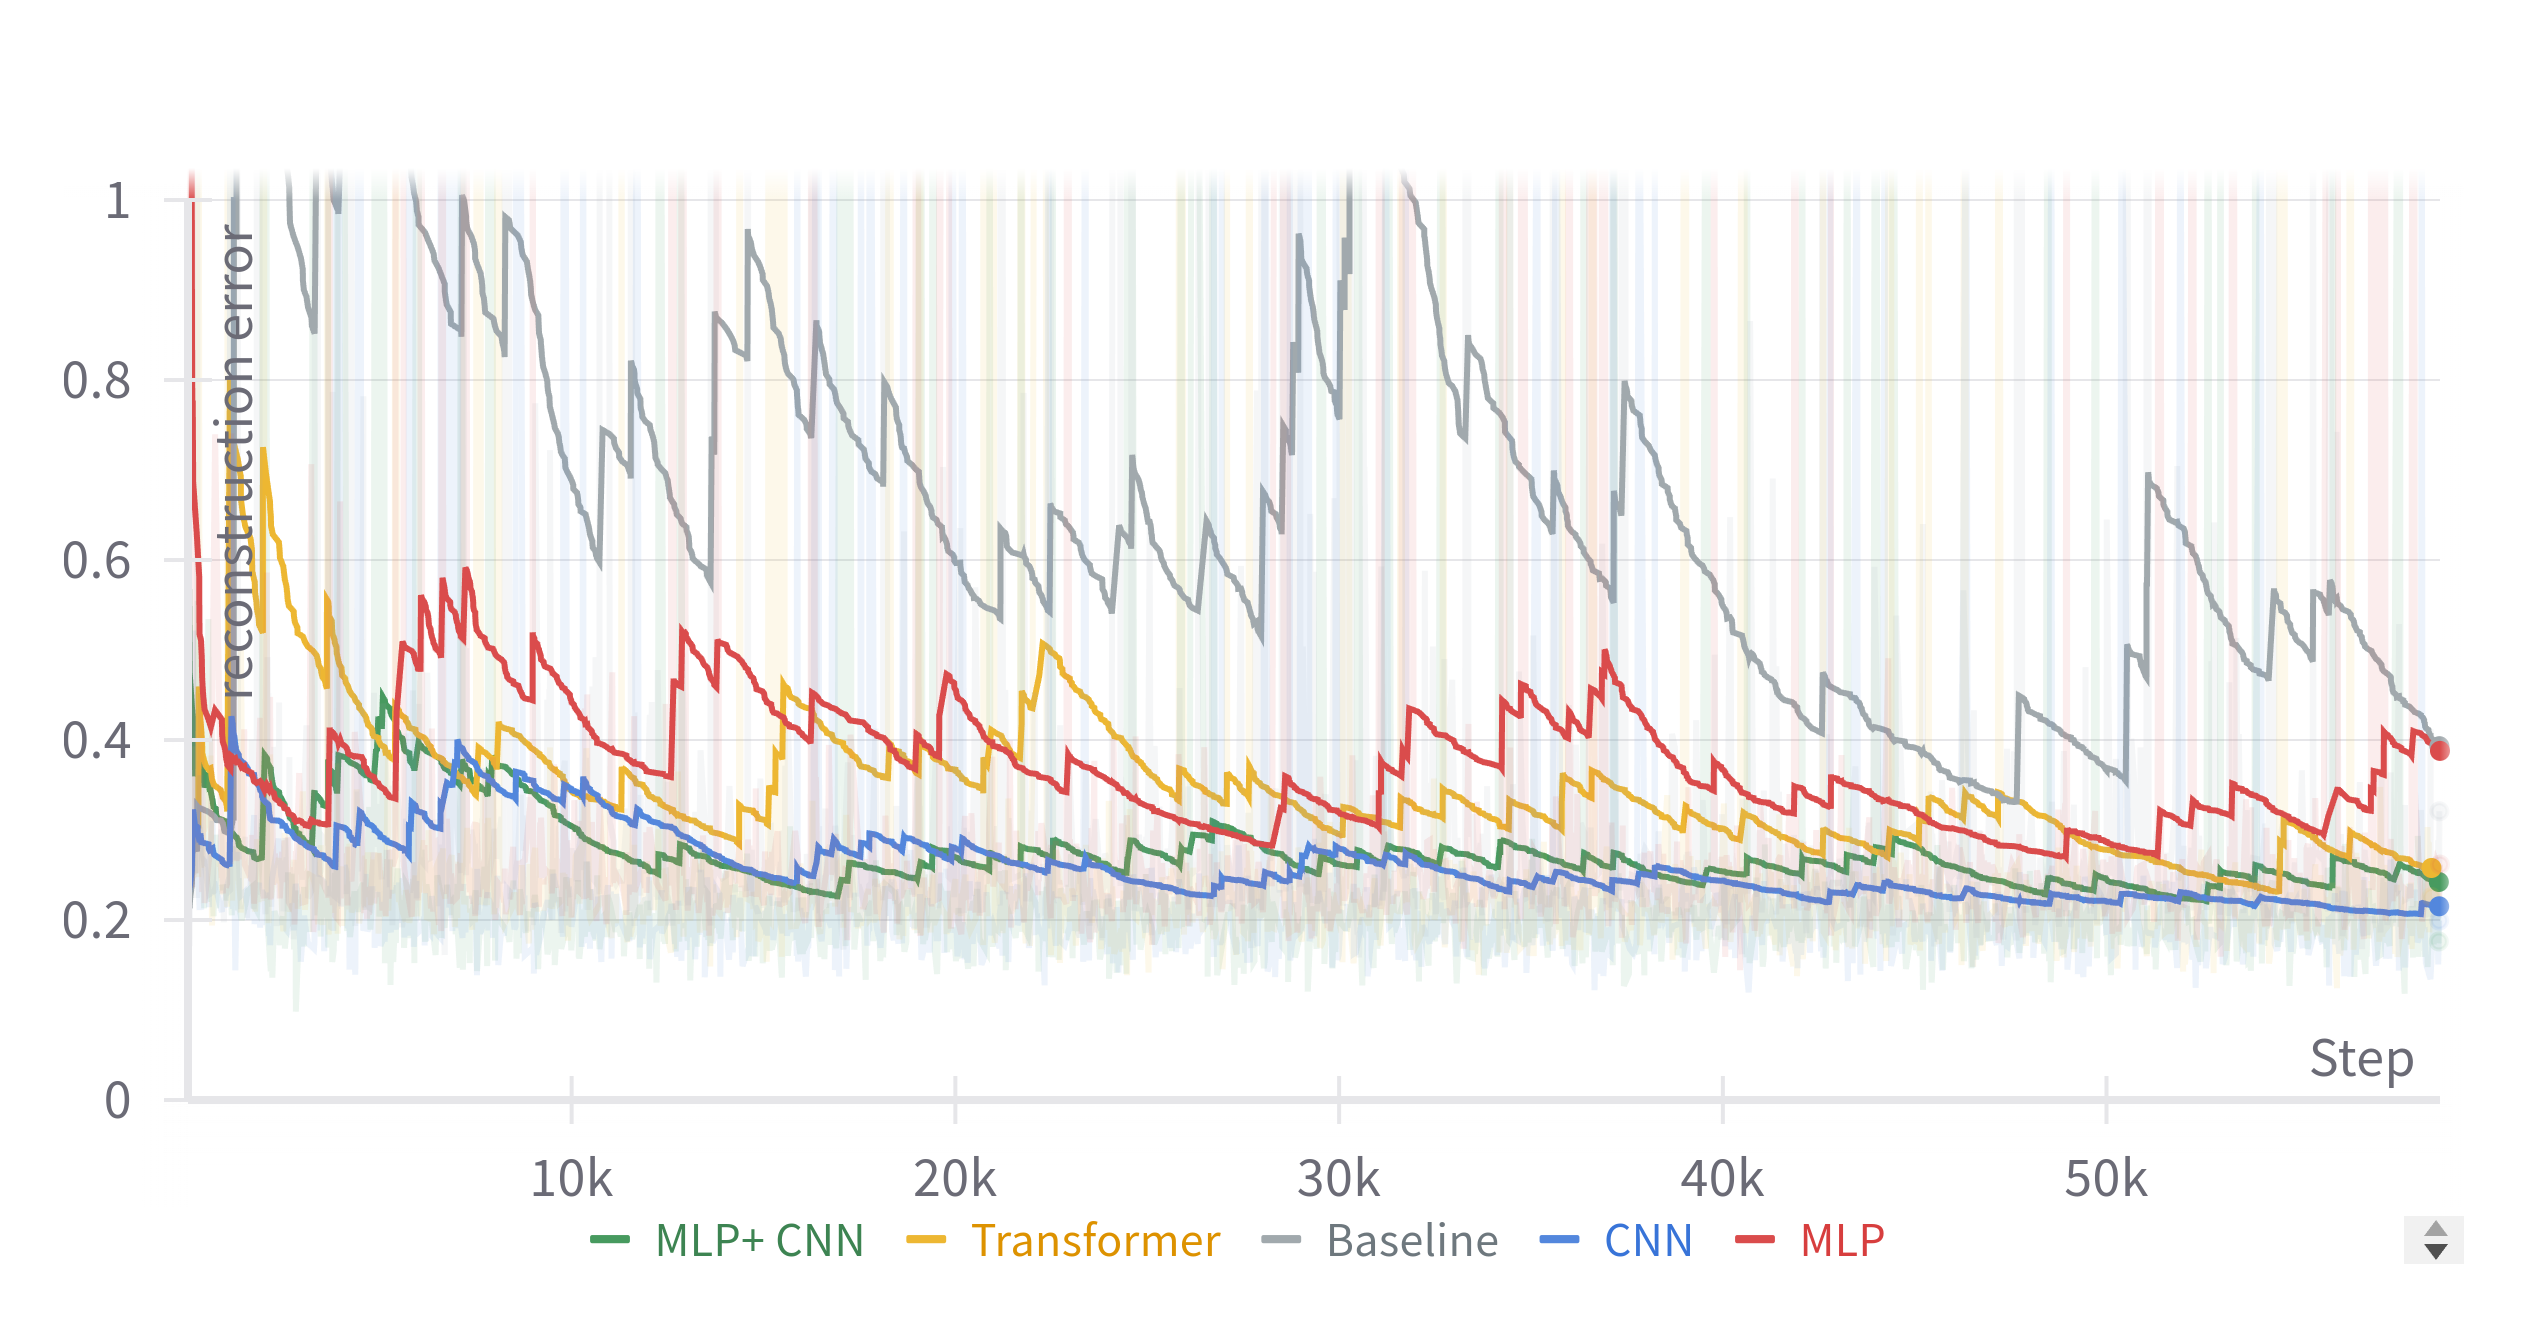
\includegraphics[width = 0.25\textwidth]{figures/recerrortrain.png}}
  \subfloat[validation rec error]{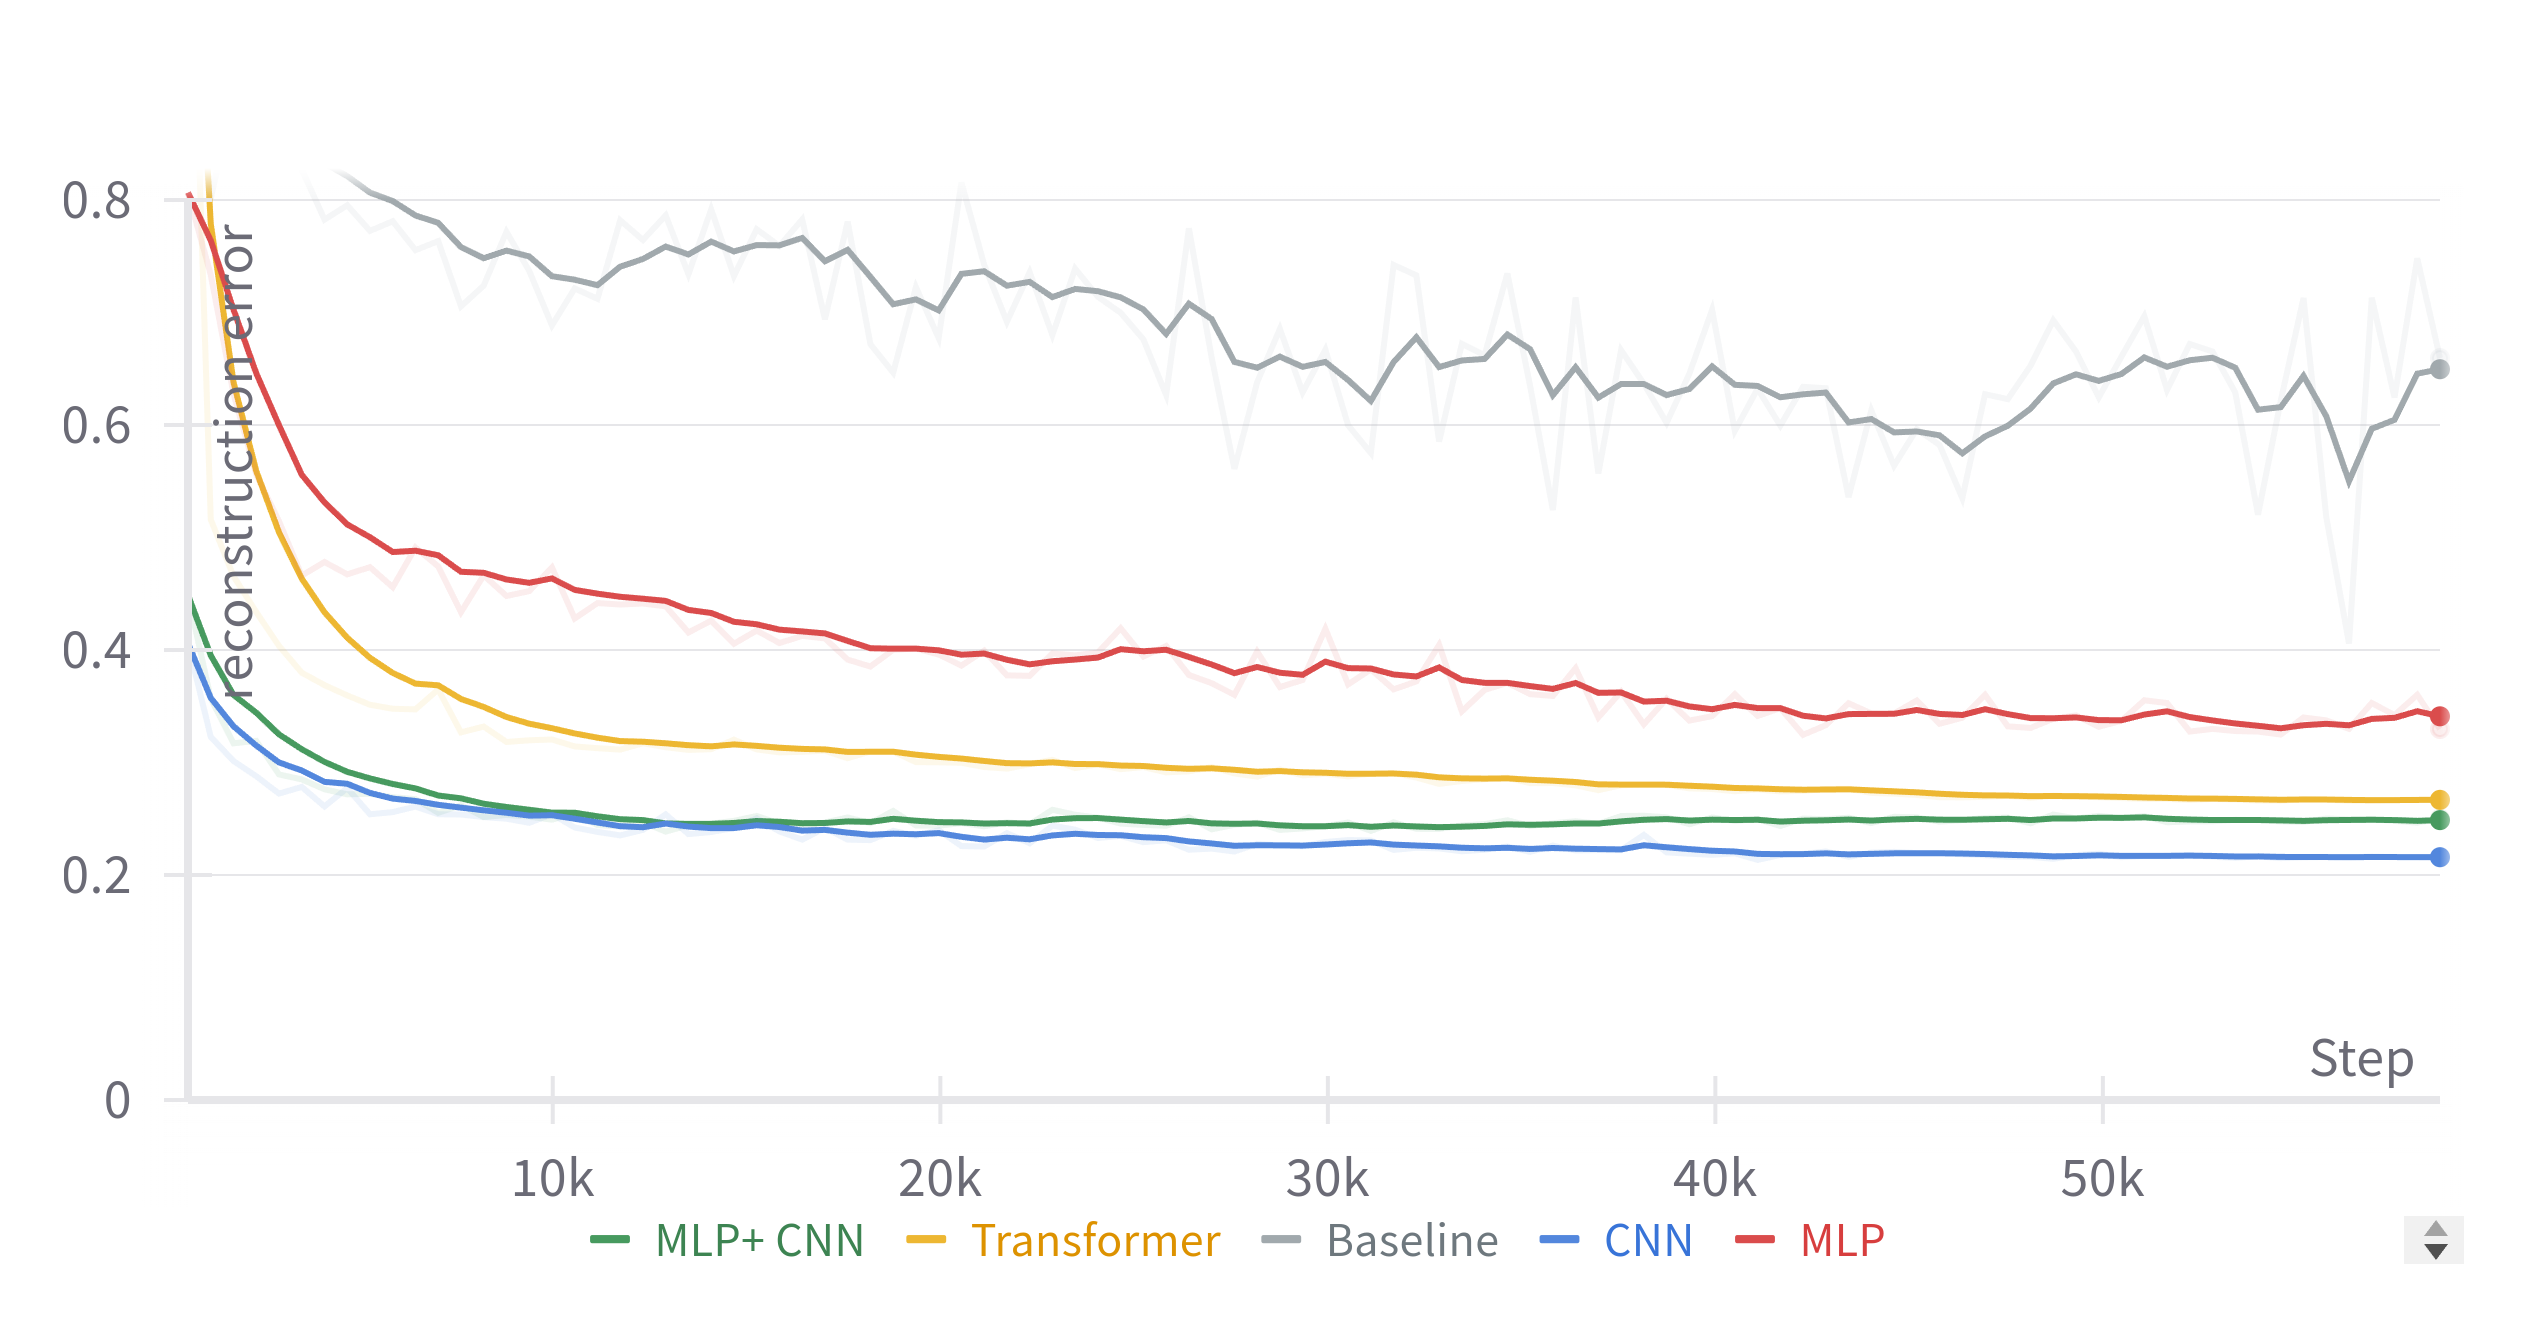
\includegraphics[width = 0.25\textwidth]{figures/recerrorval.png}}

  \caption{Top curves are smoothed loss curves for all diffusion model architectures during training on train and validation data. Bottom curves are smoothed reconstruction error e.g. $||x_p,x||$ during training and validation using single shot denoising according to Eq \ref{eq:denoise}.}
  \label{fig:losscurvesall}
\end{wrapfigure}

\begin{figure}
    \centering
    \subfloat[CNN]{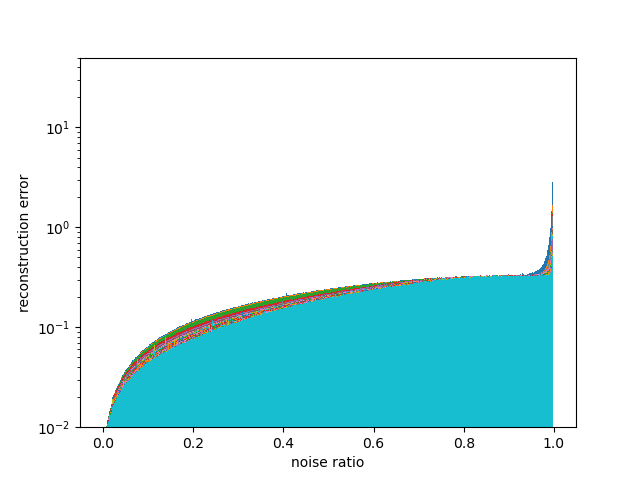
\includegraphics[width = 0.33\textwidth]{figures/Cnn.png}}
    \subfloat[Transformer]{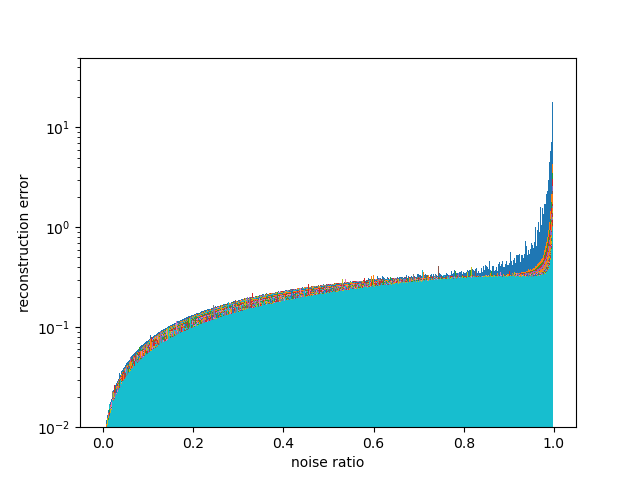
\includegraphics[width = 0.33\textwidth]{figures/Transformer.png}}  
    \subfloat[MLP]{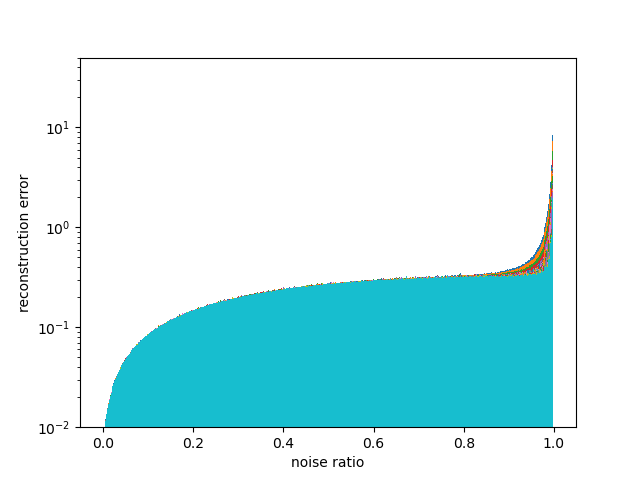
\includegraphics[width = 0.33\textwidth]{figures/MLP.png}}  

    
    \caption{Reconstruction error vs noise curves during training for different diffusion model backbones. Note the logarithmic scaling of the y-axis. }
    \label{fig:lossvsnoise}
\end{figure}



\subsection{Evaluation}

\begin{wrapfigure}{r}{0.5\textwidth}
  \centering
  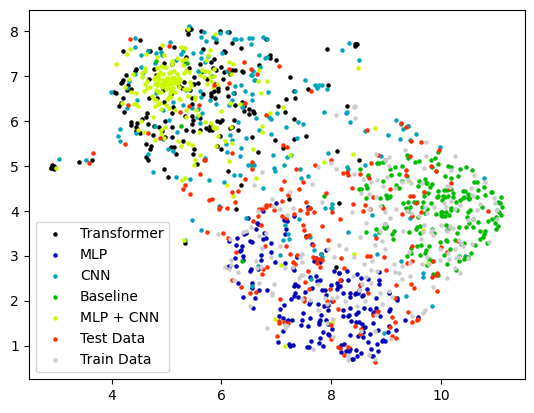
\includegraphics[width = 0.48\textwidth]{figures/umap.png}
  \caption{UMAP visualizations of data of different origins. Red and grey points are test and train data (real). Blue is MLP, green is Baseline. Yellow, black and bright blue are MLP + CNN, Transformer and CNN respectively.}
  \label{fig:umap}
\end{wrapfigure}
Next we take a closer look at the performance of a classifier trained on synthetic vs real data, see Table \ref{Fig:cls}. We observe the MLP generated data performing superior compared to all other synthetic data types with around $84.7\%$ accuracy, whereas the CNN based data fails to capture the relations important for ALS classification with the best performance of $62.64\%$ and the Transformer generated data having a maximum accuracy of $64.62\%$ on the real test data.
Training on real data is performing best with $87.6\%$ accuracy, as expected.

% \begin{figure}[t]
%     \centering
%     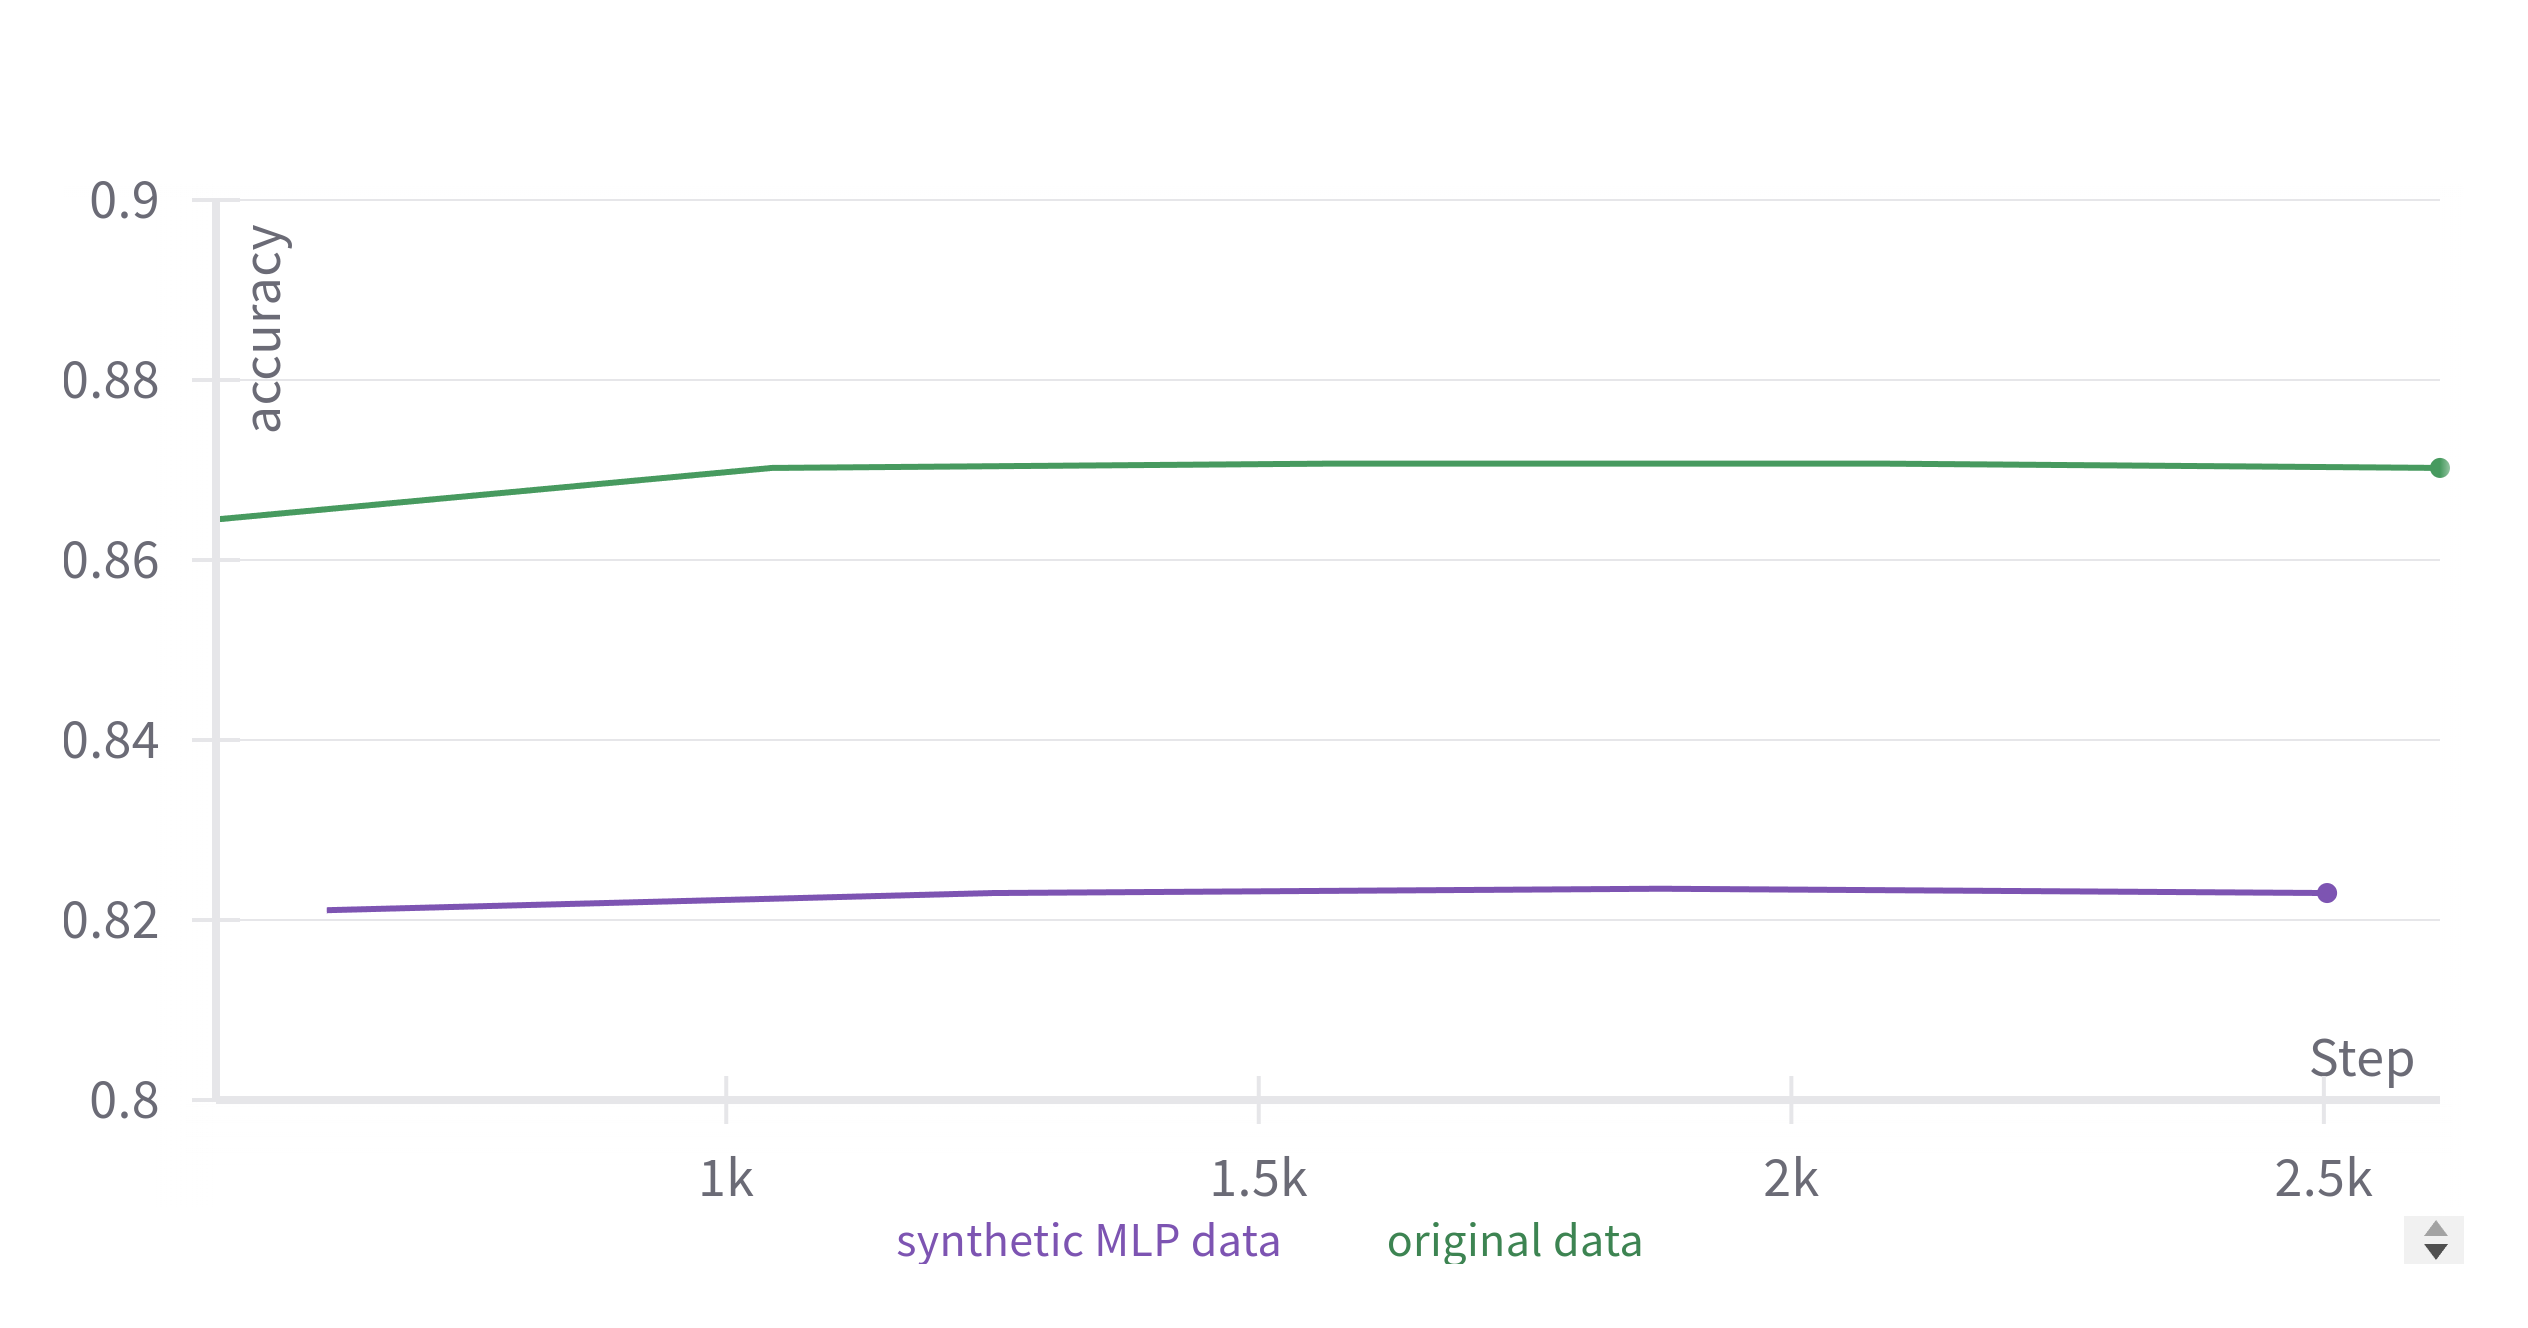
\includegraphics[width = 0.48\textwidth]{figures/test_acc.png}
%     \caption{Test accuracy on MLP generated and Baseline data. CNN generated data not visualized due to poor performance.}
%     \label{fig:cls}
% \end{figure}

\begin{table}
  \centering
  \caption{Accuracy on a hold out test set after training different ALS classifier (MLP, Transformer or CNN)  on different synthetically generated data types (generated by: MLP, Transformer, CNN, MLP + CNN or Baseline). The best synthetic data for each classifier type is marked in \textbf{bold}.}
  \label{Fig:cls}
  \begin{tabular}{c|cccccc}
    \toprule
Classifier & Real Data  & CNN  & MLP  & MLP + CNN & Transformer & Baseline \\
 
   \cmidrule(r){1-7} 
MLP &  87.60 & 62.64 & \textbf{84.71} & 82.21 & 64.62 & 70.19 \\
Transformer & 82.11  & 54.23 &  \textbf{76.73} & 71.06 & 56.92 & 45.10 \\
CNN &  73.17 & 51.15 & \textbf{67.11} & 50.00 & 50.29 & 50.00 \\
\cmidrule(r){1-7} 
average & 80.79 & 56.01 & \textbf{76.18} & 66.01 & 57.28 & 55.10\\
    \bottomrule
  \end{tabular}
\end{table}



% In Table \ref{Fig:nndistance}, we show the results of the nearest neighbour score. One possibility for the diffusion model to produce convincing results is by reproducing the data it was trained on. To rule out this possibility we take a closer look at the nearest neighbour score. We compute this score from the original training distribution $D$ to itself as a Baseline and to the data generated by the MLP and the CNN model. We observe that while the CNN has a lower distance than the baseline, which indicates some possibility of reproduction, our more successful MLP model actually has a very high score, which indicates a very diverse set of newly generated data points.

% \begin{table}
%   \centering
%   \caption{Result of nearest neighbour score for datasets generated by the MLP as well as the CNN models as well as a baseline.}
%   \label{Fig:nndistance}
%   \begin{tabular}{ cccc}
%     \toprule
% Baseline  & CNN & MLP & Transformer  \\
 
%   \cmidrule(r){1-4} 
%  63293 & 79168 & 70261 &  \\


%     \bottomrule
%   \end{tabular}
% \end{table}

% \begin{table}
%   \centering
%   \caption{Result of Nearest Neighbour adversarial accuracy for datasets generated by the MLP as well as the CNN models as well as a baseline.}
%   \label{Fig:nndistance}
%   \begin{tabular}{c cc}
%     \toprule
%   & CNN & MLP  \\

%   \cmidrule(r){1-1}  \cmidrule(r){2-3} 
%    $AA_{truth}$ & 0.4 & 0.55 \\
%    $AA_{syn}$& 0.0 & 0.18  \\
%    $AA_{TS}$ & 0.2 & 0.365 \\
%  Privacy Loss & -0.07 & 0.015 \\


%     \bottomrule
%   \end{tabular}
% \end{table}




In Figure \ref{fig:umap}, we visualize the distribution of different data types using UMAP \citep{UMAP} with cosine distance metrics. Euclidean distance metrics are notoriously bad for high dimensional data and return uniform distributions.
%Red and grey points are real test and train data. Blue data points are generated by MLP, green ones by Baseline. Yellow, black and bright blue ones are generated by MLP + CNN, Transformer and CNN respectively.
We observe that the UnetMLP generated data is closest to the real data in the UMAP visualization. 
The Baseline generated data is close to some of the training data (grey) but comparatively little of the test data (red), indicating over-fitting on the training set, this is especially interesting as Figure \ref{fig:losscurvesall} does not indicate any over-fitting during training.
The Transformer, CNN and MLP + CNN generated points are all clustering together with only small overlap with the training or test data.
Even though this UMAP visualization can give us an indication of neighbourhood structure, we want to emphasize that the visualizations can be highly misleading. In this example, MLP + CNN and CNN generated points are similarly visualized while the classification task performance, see Table \ref{Fig:cls}, is very different in between both groups. 
%Real Training data is red, validation data is brown, CNN generated data is blue and MLP generated data is green. No clear clusters seem to be forming, neither according to the baseline classes of ALS positive/negative or due to the origin of the data. Thereby we conclude that either UMAP is not able to discern complex relationships and/or the generated data is of sufficient quality to be similar enough.



Next we look at the nearest neighbour test and the nearest neighbour adversarial accuracy, see Tables \ref{Fig:nnacc} and \ref{Fig:nntest}. We observe MLP+CNN performing best for the nearest neighbour test and CNN performing best for nearest neighbour adversarial accuracy. While these test shed some light on the quality of the generated data, we do not think that distance metrics on the high dimensional input data are especially meaningful. This strongly reduces the value of these tests.


\begin{table}
  \centering
  \caption{Result of nearest neighbour test (k=10) for all datasets. Closer to 0.5 is better. Best performance is marked in \textbf{bold}.}
  \label{Fig:nntest}
  \begin{tabular}{c|ccccc}
    \toprule
comparison data &  CNN & MLP & MLP + CNN &Transformer & Baseline \\
   \cmidrule(r){1-6} 
train & 0.7835 & 0.0165 & \textbf{0.4039} & 0.7935 & 0.0265  \\
test &  0.7755 & 0.2825 & \textbf{0.3740} & 0.765 & 0.3515 \\


    \bottomrule
  \end{tabular}
\end{table}

\begin{table}
  \centering
  \caption{Result of Nearest Neighbour adversarial accuracy for generated datasets. Closer to 0.5 is better. Best performance is marked in \textbf{bold}.}
  \label{Fig:nnacc}
  \begin{tabular}{c ccccc}
    \toprule
  & CNN & MLP  & MLP + CNN & Transformer & Baseline \\

  \cmidrule(r){1-1}  \cmidrule(r){2-6} 
   $AA_{truth}$ & 0.755 & 0.225  & \textbf{0.415} & 0.915 & 0.35\\
   $AA_{syn}$& \textbf{0.62} & 1.0  & 0.925 &  0.65 & 0.995 \\
  % $AA_{TS}$ & 0.6875 & 0.6125  & 0.67 &  0.7825 & 0.6725 \\
% Privacy Loss & -0.07 & 0.015 \\


    \bottomrule
  \end{tabular}
\end{table}